\documentclass{beamer}
\usetheme{Boadilla}
% \renewcommand{\baselinestretch}{1.5}

\usepackage{physics} % better derivative writings
\usepackage{unicode-math}

\NewDocumentCommand{\e}{}{\symrm{e}}

\title{Maclaurin Series}
\author{Kutay}
\institute{Made with LaTeX}
\date{\today}

% \parskip=10pt

% \setkomafont{disposition}{\normalfont\bfseries}

\begin{document}

\begin{frame}
  \titlepage
\end{frame}

\begin{frame}
  \frametitle{Outline}
  \tableofcontents
\end{frame}

\section{What is it?}

\begin{frame}
  \frametitle{What is it?}
  \begin{itemize}
    \item Approximation of a function with an infinite series
    \item Approximates near 0
  \end{itemize}
\end{frame}

\section{Why?}

\begin{frame}
  \frametitle{Why?}
  \begin{itemize}
    \item To compute \( \sin x \), \( \cos x \), and \( \e^x \) \textit{fast}
    \item Calculators (your TI) use this technique
    \item To simplify equations/functions
    \item In simple pendulum, we \textit{approximated} \( \sin x \) with \( x \)
  \end{itemize}
\end{frame}

\section{Derivation}

\begin{frame}
  \frametitle{Derivation}
  \begin{itemize}
    \item Calculators can multiply, add, subtract, divide, and take powers of whole numbers \textit{quickly}
    \item Let us use \textit{polynomials}
    \item Polynomials are just multiplications, additions, and exponentiations
  \end{itemize}
\end{frame}

\begin{frame}
  \frametitle{Derivation}
  \begin{equation*}
    \cos x
  \end{equation*}
  \begin{figure}[ht]
    \centering
    \caption{The Function \( \cos x \)}
    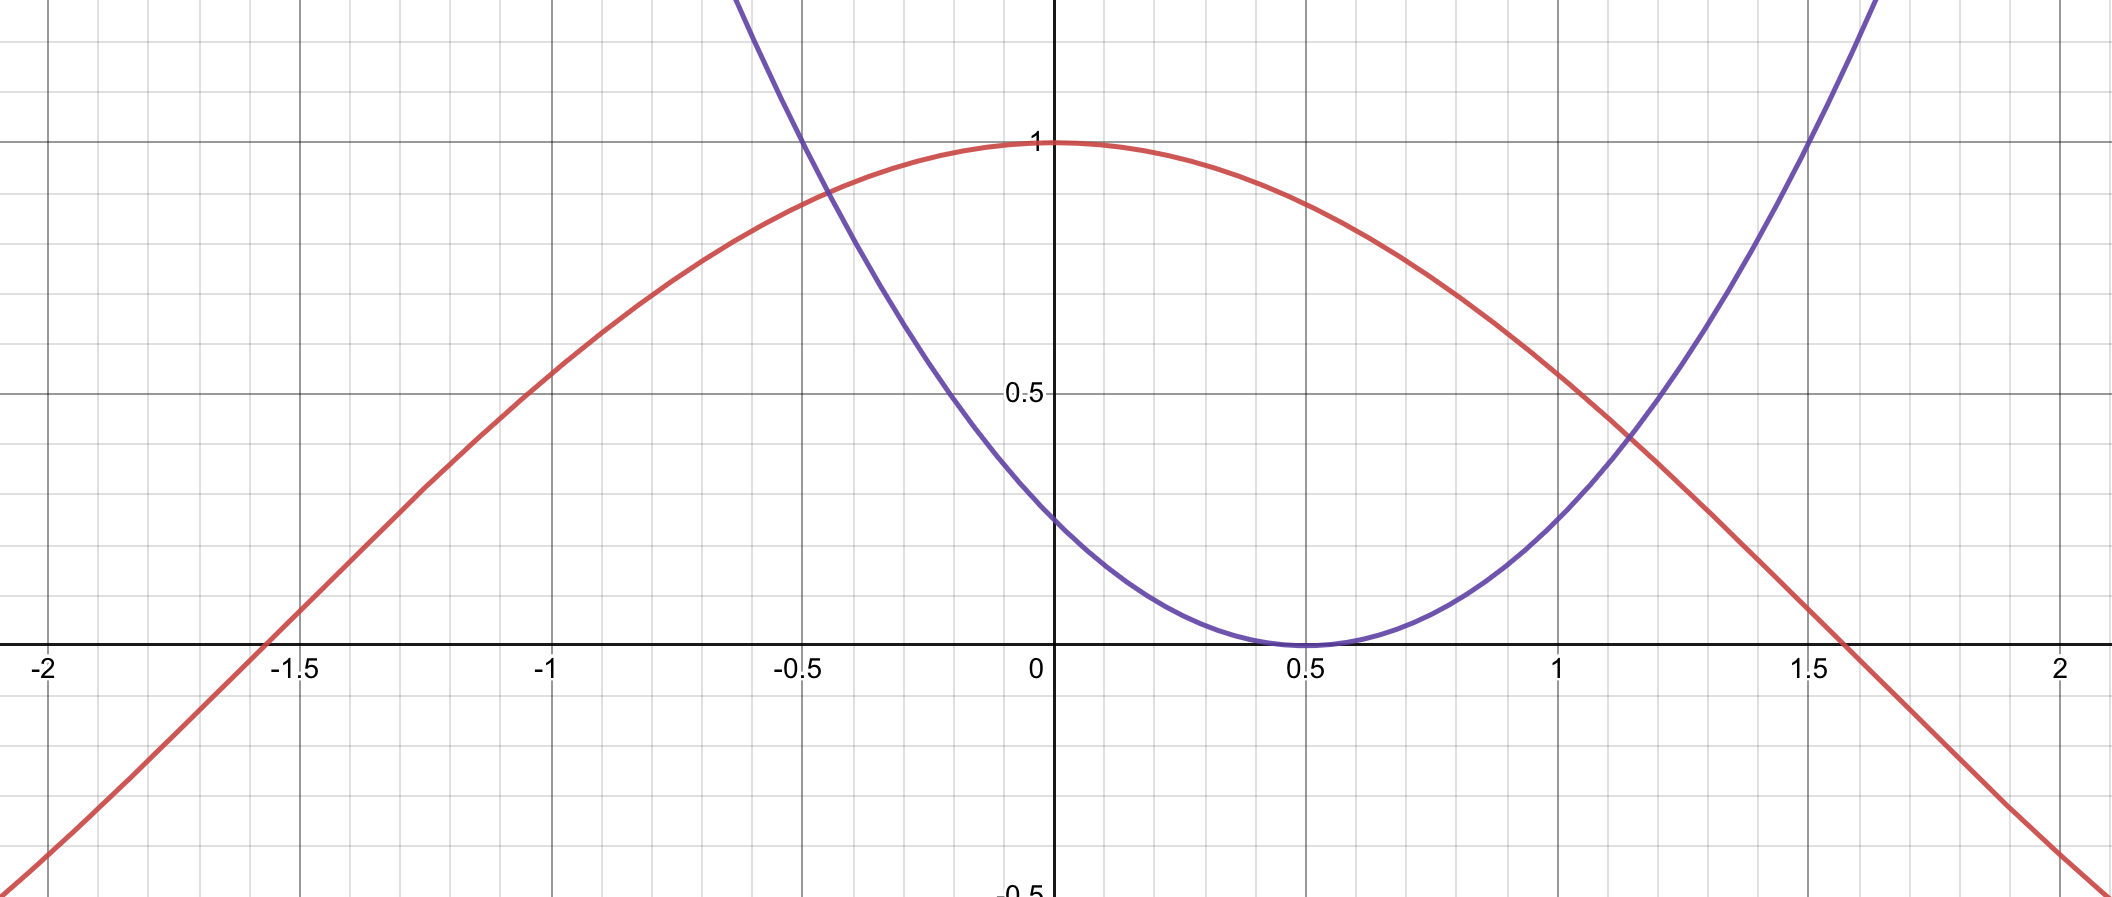
\includegraphics[
      scale=0.5
    ]{images/cosx.png}
  \end{figure}
  \begin{itemize}
    \item Approximate to two degrees
    \item Find real numbers for \( a, b, \) and \( c \)
  \end{itemize}
  \begin{equation*}
    \cos x \approx a + bx + cx^2
  \end{equation*}
\end{frame}

\end{document}
